%Tipo de documento ABNTEX2
\documentclass[12pt,openright,oneside,a4paper,
chapter=TITLE,  % títulos de capítulos convertidos em letras maiúsculas
section=TITLE,  % títulos de seções convertidos em letras maiúsculas
subsection=TITLE, % títulos de subseções convertidos em letras maiúsculas
subsubsection=TITLE, % títulos de subsubseções em letras maiúsculas
subsubsubsection=TITLE, % títulos de subsubsubseções em letras maiúsculas
english,french,spanish,brazil]{abntex2}
%É interessante observar que a ABNT NBR 14724:2011 (seção 5.1) recomenda que os documentos sejam impressos no anverso e no verso das folhas. Isso é obtido com a opção twoside.

%+++++++++++++++++++++++++++++++++++++++++++++++++++++++++++++++++++++
%Pacotes para língua portuguesa do Brasil:
\usepackage{ifxetex}
\ifxetex
    \usepackage{fontspec}
    \defaultfontfeatures{Ligatures={TeX}}
\else
    \usepackage[utf8]{inputenc}
    \usepackage[T1]{fontenc}
\fi

%Observação: Quando um documento é compilado com xelatex, os pacotes inputenc e fontenc não devem ser incluídos ao preâmbulo do documento. Ao invés desses pacotes, geralmente fontspec é usado. O código anterior de preâmbulo torna flexível a compilação do documento, que pode tanto ser realizada da forma tradicional com pdflatex quanto com xelatex, uma vez que inclui seletivamente os pacotes adequados para cada compilador (página 14 do link http://mirror.hmc.edu/ctan/macros/latex/contrib/abntex2/doc/abntex2.pdf).

%+++++++++++++++++++++++++++++++++++++++++++++++++++++++++++++++++++++
%In formações do projeto de TCC:
\titulo{Projeto De Um Robô Móvel Integrando Raspberry Pi com o Sistema De Visão Computacional OPENCV}
\autor{Gabriel Matias Souza Silva}
\orientador{Prof. Dr. Marcos Roberto Bombacini}
\coorientador{}
\data{2020} % Apenas o ano
\local{Toledo} % Apenas a cidade

% Não alterar o preambulo!:
\preambulo{Projeto de Trabalho de Conclusão de Curso apresentado à disciplina de Trabalho de Conclusão de Curso 1 do Curso de Engenharia Eletrônica da Universidade Tecnológica Federal do Paraná - UTFPR Campus Toledo, como requisito parcial para a obtenção do título de Bacharel em Engenharia Eletrônica.}

%+++++++++++++++++++++++++++++++++++++++++++++++++++++++++++++++++++++
%Pacotes adicionais:
\usepackage{amssymb}
\usepackage{tabto}
\usepackage{hyperref}
\usepackage[%
    alf,
    abnt-emphasize=bf,
    bibjustif,
    recuo=0cm,
    abnt-url-package=url,       % Utiliza o pacote url
    abnt-refinfo=yes,           % Utiliza o estilo bibliográfico abnt-refinfo
    abnt-etal-cite=3,
    abnt-etal-list=3,
    abnt-thesis-year=final
]{abntex2cite} 
\usepackage{graphicx}
\usepackage{nomencl} % Para a lista breviaturas e siglas
\makenomenclature    % Para a lista breviaturas e siglas

%+++++++++++++++++++++++++++++++++++++++++++++++++++++++++++++++++++++
%insira novos pacotes aqui:
\usepackage{indentfirst} % Indenta o primeiro parágrafo de cada seção.
\usepackage{multirow} % Pacote de tabulação para tabelas
\usepackage{bm}
\usepackage{lastpage} % Usado por abntex2-fichacatalografica.tex
\usepackage[font=small,labelfont=bf,textfont=bf]{caption} % Legendas de floats em tamanho 10pt e negrito
\usepackage{listings}
\usepackage{textcomp}
\usepackage{caption}
\usepackage{upgreek}

%+++++++++++++++++++++++++++++++++++++++++++++++++++++++++++++++++++++
%Outras configurações:

% "Por padrão, uma versão sem serifas da fonte corrente do documento é utilizada para os títulos das divisões. Você pode customizar a fonte dos títulos dos capítulos alterando os comandos como no exemplo a seguir, para que seja utilizada a fonte Computer Modern com tamanho maior do que o utilizado por padrão" (manual do abntex2).
\renewcommand{\ABNTEXchapterfont}{\fontfamily{cmr}\fontseries{b}\selectfont}
\renewcommand{\ABNTEXchapterfontsize}{\HUGE}

% Para criação de quadros
% Novo list of (listings) para QUADROS

\newcommand{\quadroname}{Quadro}
\newcommand{\listofquadrosname}{Lista de quadros}

\newfloat[chapter]{quadro}{loq}{\quadroname}
\newlistof{listofquadros}{loq}{\listofquadrosname}
\newlistentry{quadro}{loq}{0}

% configurações para atender às regras da ABNT
\setfloatadjustment{quadro}{\centering}
\counterwithout{quadro}{chapter}
\renewcommand{\cftquadroname}{\quadroname\space} 
\renewcommand*{\cftquadroaftersnum}{\hfill--\hfill}

% Configuração de posicionamento padrão:
\setfloatlocations{quadro}{hbtp}

% Abreviação de microcontrolador
\newcommand{\micro}{$\mathrm{\upmu C}$}

%\setlength\afterchapskip{\lineskip} // Espaçamento de 1,5 entre o título do capítulo e corpo do texto

%+++++++++++++++++++++++++++++++++++++++++++++++++++++++++++++++++++++
%Início do documento:
\begin{document}

    %+++++++++++++++++++++++++++++++++++++++++++++++++++++++++++++++++
    % Elementos pré-textuais
    \pretextual

    % Imprime capa e pula sua numeração
    \pagenumbering{gobble} % Remove a visualização da numeração das páginas e reinicia em 1 
    \clearpage
    \thispagestyle{empty}
    \imprimircapa
    \clearpage
    \pagenumbering{arabic}% Numeração arábica (e reinicia em 1)

    % Imprime a folha de rosto (padrão do abntex2)
    \imprimirfolhaderosto*

    % Insere a ficha catalográfica (Obrigatório)
    %\begin{fichacatalografica}
    \sffamily
    \vspace*{15cm}    % Posição vertical
    \hrule       % Linha horizontal
    \begin{center}    % Minipage Centralizado
        \begin{minipage}[c]{12.5cm} % Largura
            \imprimirautor
            \hspace{0.5cm} \imprimirtitulo / \imprimirautor. --
            \imprimirlocal, \imprimirdata-
            \hspace{0.5cm} \pageref{LastPage} p. : il.(alguma color.); 30 cm.\\
            \hspace{0.5cm} \imprimirorientadorRotulo \imprimirorientador\\
            \hspace{0.5cm}
            \parbox[t]{\textwidth}{\imprimirtipotrabalho~--~\imprimirinstituicao,
            \imprimirdata.}\\
            \hspace{0.5cm}
            1. Palavra-chave1.
            2. Palavra-chave2.
            I. Orientador.
            II. Universidade xxx.
            III. Faculdade de xxx.
            IV. Título\\
            \hspace{8.75cm} CDU 02:141:005.7\\
        \end{minipage}
    \end{center}
\hrule
\end{fichacatalografica}

    % Insere a folha de aprovação
    %\begin{folhadeaprovacao}
    \begin{center}
        {\ABNTEXchapterfont\large\imprimirautor}
        \vspace*{\fill}\vspace*{\fill}
            \begin{center}
                \ABNTEXchapterfont\bfseries\Large\imprimirtitulo
            \end{center}
            \vspace*{\fill}
            \hspace{.45\textwidth}
            \begin{minipage}{.5\textwidth}
                \imprimirpreambulo
            \end{minipage}%
            \vspace*{\fill}
    \end{center}
    Trabalho aprovado. \imprimirlocal, 24 de novembro de 2012:
    \assinatura{\textbf{\imprimirorientador} \\ Orientador}
    \assinatura{\textbf{Professor} \\ Convidado 1}
    \assinatura{\textbf{Professor} \\ Convidado 2}
    
    \begin{center}
        \vspace*{0.5cm}
        {\large\imprimirlocal}
        \par
        {\large\imprimirdata}
        \vspace*{1cm}
    \end{center}
\end{folhadeaprovacao}

    % Insere o resumo em pt-br
    %\chapter*{Resumo}

% --- resumo em português ---
\begin{resumo}
A maior parte dos sistemas de visão artificial desenvolvidos nos dias atuais utiliza duas câmeras para o sensoriamento. Esta técnica é conhecida como sistema de visão estereoscópica binocular. Nela são utilizadas duas imagens dispostas em diferentes posições para determinar a estrutura tridimensional dos objetos, utilizando o princípio da triangulação. O princípio da triangulação determina a posição do objeto através da intersecção dos raios correspondentes à projeção na imagem de cada câmera e tem como maior dificuldade identificar os elementos correspondentes nas duas imagens, sendo conhecido como o problema da correspondência estereoscópica. 

Em grande parte, os problemas inerentes de um sistema de visão computacional dependerão de sua aplicação, do tipo de informação relevante da imagem, da metodologia para obter essa informação e quais ações o robô irá tomar a partir disto.

Uma vez que, a informação tridimensional pode ser obtida utilizando apenas uma câmera e um sensor que obtenha uma informação de distância do objeto. Sendo assim, essa técnica proporciona um menor tempo de processamento, o que para um robô móvel é de suma importância. Este projeto de conclusão de curso tem como objetivo implementar um algoritmo de controle em um microcontrolador Raspberry Pi. Este hardware será embarcado em um robô móvel que terá entradas oriundas de sensores ultra-sônicos e  de uma câmera permitindo a identificação do ambiente de maneira autônoma.

\vspace{\onelineskip}
\noindent
\textbf{Palavras-chave}: robô móvel, raspberry pi, arduino, visão computacional, opencv.
\end{resumo}

% --- resumo em inglês ---
% \begin{resumo}[Abstract]
%     \begin{otherlanguage*}{english}
%         Abstract here.
        
%         \vspace{\onelineskip}
%         \noindent
%         \textbf{Keywords}: latex. abntex. publication de textes.
%     \end{otherlanguage*}
% \end{resumo}


 %resumo (deve conter resumo)

    %Lista de figuras
    \pdfbookmark[0]{\listfigurename}{lof}
    \listoffigures* 
    \cleardoublepage

    %Lista de tabelas
    %\listoftables

    %lista de abreviaturas e siglas
    \renewcommand{\nomname}{\listadesiglasname}
    \pdfbookmark[0]{\nomname}{las}
    \printnomenclature
    \cleardoublepage

    % Lista de símbolos
    % Inserir os símbolos em ordem alfabética

%\begin{simbolos}

    
%\end{simbolos}

%\item[$ n $] Índice de refração do núcleo de uma fibra óptica
%\item[$ n_{cl} $] Índice de refração do revestimento de uma fibra óptica
%\item[$\Delta n$] Amplitude de perturbação do índice de refração induzida
%\item[$\Lambda$] Período da grade de Bragg
%\item[$z$] Distância coaxial da fibra
%\item [$\hslash$] Constante de Planck
%\item[$\omega_r$] Frequência angular refletida
%\item[$\omega_i$] Frequência angular incidente 
%\item[$\bm{k_i}$] Vetor de onda incidente
%\item[$\bm{k_r}$] Vetor de onda refletido
%\item[$k$] Vetor de onda da grade
%\item[$\pi$] Pi
%\item[$\Delta l$] Deformação da fibra óptica
%\item[$\Delta T$] Variação da temperatura
%\item[$p_\varepsilon$] Constante efetiva tensão-óptica
%\item[$\varepsilon$] Deformação da fibra
%\item[$\alpha_\Lambda$] Coeficiente de expansão térmica 
%\item[$\alpha_n$] Coeficiente termo-óptico
%\item[$\lambda_0$] Comprimento de onda central do laser
%\item[$T_0$] Temperatura do laser




    %Sumário
    \pdfbookmark[0]{\contentsname}{toc}
    \tableofcontents*
    \cleardoublepage
    
    %+++++++++++++++++++++++++++++++++++++++++++++++++++++++++++++++++
    % Elementos textuais
    \textual

    \chapter{Introdução}
%\setlength{\afterchapskip}{-\baselineskip} // Espaçamento de 1,5 entre o título do capítulo e corpo do texto
\label{chap:intro}

Os sistemas de visão computacional estão presentes em diversas áreas, sendo elas medicina, análise de impressões digitais, sensoriamento remoto, robótica móvel, entre outras. O sucesso obtido pelo seu grande poder de utilização tem sido relevante para o constante desenvolvimento destas tecnologias.

Vale trazer uma definição clássica: "Visão computacional é a ciência e tecnologia das máquinas que enxergam. Ela desenvolve teoria e tecnologia para a construção de sistemas artificiais que obtém informação de imagens ou quaisquer dados multi-dimensionais"~\cite{antonello2014introduccao}.

Visão computacional foi definida como sendo o conjunto de técnicas computacionais para estimar ou explicitar as propriedades geométricas e dinâmicas do mundo tridimensional a partir de imagens \cite{alves2005estudo}.

Devido a crescente automatização dos processos produtivos, busca-se tornar os sistemas computacionais e de robótica capazes de tornar automática a execução de tarefas complexas \cite{rudek2001visao}.

Sabe-se que a visão é a principal forma de obtenção de informações do ambiente para a maioria dos seres vivos. A imagem é formada na mente a partir dos olhos, que funcionam como sensores de luminosidade, e é processada pelo cérebro que determina a ação a ser tomada. Por exemplo, em um movimento para se pegar um copo a visão tem papel fundamental junto com a coordenação motora \cite{alves2005estudo}. É perceptível que muitas ações realizadas no dia a dia são extremante complicadas de se fazer sem o advento da visão.

Para visão computacional, em lugar de olhos temos câmeras como sensores de obtenção de imagens digitais. Estas imagens passam por um processamento digital onde técnicas computacionais tiram as informações desejadas do ambiente, variando de acordo com o objetivo da aplicação. Para a robótica, é comum a utilização na identificação de objetos, localização e locomoção. Diversas técnicas de reconhecimento de imagens, tem sido apresentadas na literatura e geralmente são validadas através de protótipo de aplicações, pois em um ambiente industrial, raramente obtém-se as condições ideais de iluminação, contraste, posicionamento correto da peça, e do ângulo de obtenção da imagem, além de outros fatores externos que dificultam a interpretação de uma cena. Uma imagem digital pode conter várias informações, que deverão ser tratadas em diferentes etapas da produção. Estas informações impossibilitam que imagens diferentes possam ser tratadas de uma forma única, isto é, imagens diferentes possuem requisitos de programação diferentes \cite{rudek2001visao}.

Portanto, temos a primeira etapa de desenvolvimento e utilização de um sistema de visão computacional, a definição do problema. Essa e as demais etapas serão apresentadas no Capítulo~\ref{chap:refteorico}.

%================================================================================
\section{Justificativa}
\label{sec:justi}

Este projeto visa dotar o robô com visão computacional e torná-lo autônomo, reduzindo o custo de uma câmera presente no sistema tradicional de triangulação.

%================================================================================
\section{Objetivos}
\label{sec:objt}

O principal objetivo deste trabalho é projetar e implementar um sistema de visão artificial computacional para um robô móvel autônomo (RMA). Desse modo, há outros objetivos que compõem este trabalho. Estes objetivos específicos são:

\begin{itemize}
    \item Desenvolver um algoritmo de processamento de imagens e implementá-lo no Raspberry Pi;
    \item Desenvolver um algoritmo de controle e implementá-lo no Arduino;
    \item Construir e testar um robô móvel autônomo.
\end{itemize}







 %introdução (deve conter objetivos e justificativa)
    \chapter{Referencial Teórico}
\label{chap:refteorico}

Nesta seção será apresentada o embasamento teórico para desenvolvimento do projeto.

%================================================================================
\section{Sistemas de Visão Computacional}
\label{sec:sistemasVisaoArtificial}

Os sistemas de visão computacional estão presentes em diversas áreas, sendo elas medicina, análise de impressões digitais, sensoriamento remoto, robótica móvel, entre outras. O sucesso obtido pelo seu grande poder de utilização tem sido relevante para o constante desenvolvimento destas tecnologias.

Visão computacional foi definida como sendo o conjunto de técnicas computacionais para estimar ou explicitar as propriedades geométricas e dinâmicas do mundo tridimensional a partir de imagens \cite{alves2005estudo}.

Devido a crescente automatização dos processos produtivos, busca-se tornar os sistemas computacionais e de robótica capazes de tornar automática a execução de tarefas complexas \cite{rudek2001visao}.

Sabe-se que a visão é a principal forma de obtenção de informações do ambiente para a maioria dos seres vivos. A imagem é formada na mente a partir dos olhos, que funcionam como sensores de luminosidade, e é processada pelo cérebro que determina a ação a ser tomada. Por exemplo, em um movimento para se pegar um copo a visão tem papel fundamental junto com a coordenação motora \cite{alves2005estudo}. É perceptível que muitas ações realizadas no dia a dia são extremante complicadas de se fazer sem o advento da visão.

Para visão computacional, em lugar de olhos temos câmeras como sensores de obtenção de imagens digitais. Estas imagens passam por um processamento digital onde técnicas computacionais tiram as informações desejadas do ambiente, variando de acordo com o objetivo da aplicação. Para a robótica, é comum a utilização na identificação de objetos, localização e locomoção. Diversas técnicas de reconhecimento de imagens, tem sido apresentadas na literatura e geralmente são validadas através de protótipo de aplicações, pois em um ambiente industrial, raramente obtém-se as condições ideais de iluminação, contraste, posicionamento correto da peça, e do ângulo de obtenção da imagem, além de outros fatores externos que dificultam a interpretação de uma cena. Uma imagem digital pode conter várias informações, que deverão ser tratadas em diferentes etapas da produção. Estas informações impossibilitam que imagens diferentes possam ser tratadas de uma forma única, isto é, imagens diferentes possuem requisitos de programação diferentes \cite{rudek2001visao}.

Portanto, temos a primeira etapa de desenvolvimento e utilização de um sistema de visão computacional, a definição do problema. As demais etapas são: aquisição da imagem, pré-processamento, segmentação, identificação do objeto e reconhecimento de padrões, como visto na Figura~\ref{fig:acoesProcImagem}.

\begin{figure}[!hbtp]
  \centering
   \caption{Ações de Aquisição e Processamento de Imagem.}
    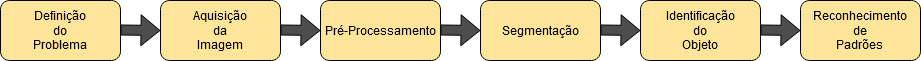
\includegraphics[width = 0.8\textwidth]{Caps/Figs/ref-teorico/acoes-procImagem.jpg}
   \label{fig:acoesProcImagem}
    \fonte{Autor}
\end{figure}

\subsection{Definição do Problema}
\label{subsec:defProblema}

Para \citeauthor{rogeralex1999} (\citeyear{rogeralex1999}), a primeira etapa do processo é a definição do problema, ou seja, qual é o objetivo que o sistema deve cumprir. Este pode ser a identificação de peças numa esteira rolante, a identificação de impressões digitais ou o reconhecimento de obstáculos na trajetória de um robô móvel. Se o sistema tiver sido bem planejado, chega-se a última etapa do processo, que é o resultado, ou seja, qual é a peça, a quem pertence a impressão digital ou qual é o obstáculo do robô.

\subsection{Aquisição da Imagem}
\label{subsec:aquisImagem}

Nesta etapa necessita-se de um dispositivo sensível a faixa do espectro eletromagnético desejado, também conhecido como câmera. Estes equipamentos que compõe o ambiente produzem em sua saída um sinal elétrico proporcional a quantidade de energia captada. Esse sinal elétrico, precisa então passar por um conversor analógico-digital para que possa ser processado pelo computador \cite{rogeralex1999}.

\subsection{Pré-processamento da Imagem}
\label{subsec:preProcImagem}

Após digitalizar e armazenar a imagem em um computador, as técnicas de pré-processamento são usadas para aprimorar a qualidade de uma imagem, corrigindo iluminação, contraste, distorções e nitidez~\cite{rudek2001visao}.

Essas operações podem ser realizadas tanto no domínio espacial quanto no domínio da frequência. O domínio espacial refere-se ao próprio plano da imagem e é caracterizado pela manipulação direta dos pixels. As técnicas de processamento no domínio da frequência são baseadas na manipulação da Transformada de Fourier da imagem~\cite{rogeralex1999}.

\subsection{Segmentação da Imagem}
\label{subsec:segImagem}

\citeauthor{heinen2004navegaccao} (\citeyear{heinen2004navegaccao}) afirma que em processamento de imagens, segmentar consiste em identificar e extrair estruturas homogêneas presentes em uma cena, sendo a eficiência deste processo diretamente relacionada ao desempenho final da análise automática de imagens. É importante enfatizar que essa é uma etapa crítica do processo.

Esta técnica é utilizada para reduzir o esforço computacional, reduzindo as informações da imagem. Para~\citeauthor{rudek2001visao} (\citeyear{rudek2001visao}), a ideia utilizada na segmentação (\textit{thresholding}) é dividir a imagem em regiões que correspondem a unidades estruturais da cena, ou que distinguem os objetos de interesse, separando os objetos da imagem (\textit{foreground}) das informações de fundo da imagem (\textit{background}). Com esta abordagem, minimiza-se o tamanho do espaço de onde as informações são retiradas, diminuindo o esforço computacional necessário para tratar a imagem.

A dificuldade normalmente encontrada está no fato de não haver conhecimento a priori do número e tipo de estruturas presentes na imagem. Estas são identificadas a partir de características como forma, geometria, topologia, textura, cor ou brilho, sendo escolhidas aquelas que possibilitam melhor distinção~\cite{heinen2004navegaccao}.

\subsection{Identificação do Objeto}
\label{subsec:idObjeto}

Visto que os elementos de interesse da imagem foram individualizados, deve-se determinar a melhor forma de representá-los, isto é, se apenas o seu contorno já contém a informação necessária ou se todos os pixels são necessários para a identificação do objeto. Portanto, deve-se determinar características do objeto que possam contribuir para a sua identificação.

\citeauthor{rudek2001visao} (\citeyear{rudek2001visao}) afirma que devido a uma variedade de razões, os dados de imagens usados na entrada de um sistema de visão, nem sempre são perfeitos. Os problemas que frequentemente ocorrem estão relacionados com a oclusão, onde um objeto pode estar parcialmente escondido atrás de outro objeto. 

De forma análoga, a perda de informações ou deformações, podem ser ocasionadas por ruídos na imagem devido a condições anormais de iluminação, defeitos de digitalização, e de resultados ineficientes de algoritmos de segmentação~\cite{beis1999indexing}.

\subsection{Reconhecimento de Padrões}
\label{subsec:recPadroes}

As técnicas de reconhecimento de padrões, tratam da identificação de partes da imagem que possuem semelhanças. Uma grande quantidade de ferramentas matemáticas e computacionais, tem sido desenvolvidas para permitir que objetos possam ser extraídos e agrupados em classes específicas de informações. Uma boa representação da forma do objeto, gera facilidades para que ele seja armazenado, transmitido, comparado, reconhecido ou mesmo entendido. A representação deve ser gerada de acordo com regras simples e precisas. Geralmente uma forma é descrita em termos de número de componentes, primitivas e relacionamentos entre estes componentes~\cite{rudek2001visao}.

%================================================================================
\section{OPENCV}
\label{sec:openCV}



%================================================================================
\section{Seção3}
\label{sec:EstimarF0}


 
 %referencial teórico
    %% =============================================================================
%% ===========      MATERIAIS E METODOS            =============================
%% =============================================================================
\chapter{Materiais e Métodos}
\label{chap:mat_met}

Nesta seção serão apresentados os materiais e métodos que serão utilizados para o desenvolvimento do projeto.

%================================================================================
\section{Visão geral do sistema proposto}
\label{sec:visaoGeralSist}

O sistema proposto consiste em um robô móvel autônomo (RMA) composto por um Raspberry Pi, um Arduino, sensores e atuadores fixados em um chassi redondo. O Raspberry Pi tem a finalidade de obter e processar a imagem a partir de um método de visão computacional da biblioteca OPENCV, adquirindo a informação necessária e transmitindo-a para o Arduino, onde o sistema de controle estará embarcado e atuará nos motores de acordo com a movimentação necessária. Um conjunto de sensores ultrassônicos será responsável pela percepção de algum objeto que poderá impedir a trajetória inicialmente definida.

Na Figura~\ref{fig:sistema-proposto} pode-se observar um esboço dos cargos de cada placa no sistema.

\begin{figure}[!hbtp]
  \centering
   \caption{Sistema Proposto}
    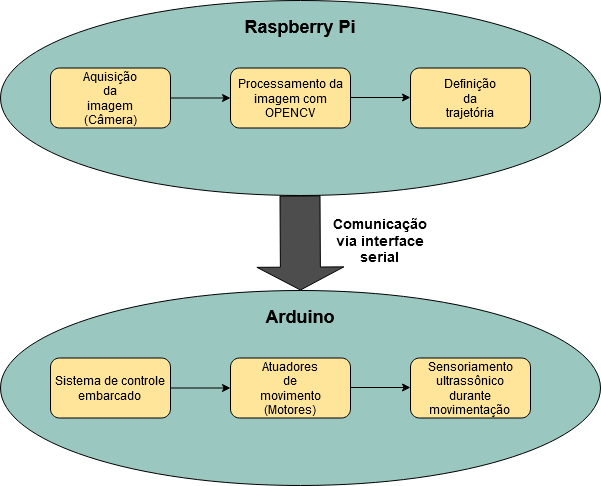
\includegraphics[width = 0.8\textwidth]{Caps/Figs/mat-met/Sistema-proposto.png}
   \label{fig:sistema-proposto}
    \fonte{Autor}
\end{figure}

\nomenclature{RMA}{Robô Móvel Autônomo}

%================================================================================
\section{Arduino}
\label{sec:Arduino}

O Arduino consiste em uma plataforma de prototipagem eletrônica com placa única e hardware livre. É projetado com um microcontrolador RISC Atmel AVR de chip único, com suporte embutido de entradas e saídas e linguagem de programação padrão que é essencialmente C/C++. Este pode receber sinais elétricos, analisá-los e tomar decisões para a ação dos atuadores a ele conectados, como relés, motores, servomotores, entre outros.

Neste projeto será utilizado um Arduino UNO, mostrado na Figura~\ref{fig:arduino-uno}, que possui 14 pinos de entrada/saída digital (dos quais 6 podem ser usados como saídas PWM), 6 entradas analógicas, um cristal oscilador de 16MHz, uma porta de conexão universal (USB - \textit{Universal Serial Bus}), uma entrada de alimentação e um botão de reset.

\begin{figure}[!hbtp]
  \centering
   \caption{Arduino UNO}
    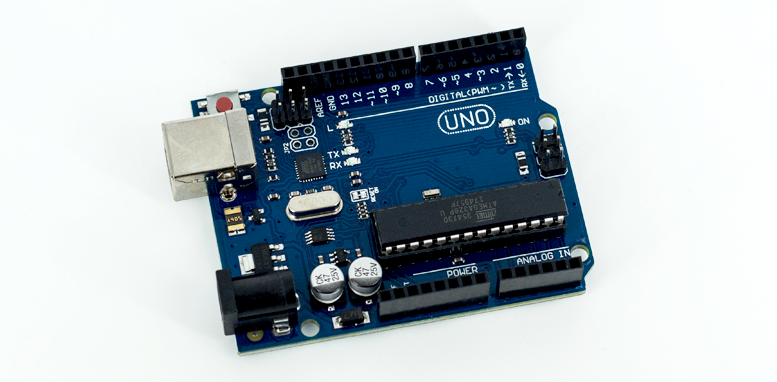
\includegraphics[width = 0.8\textwidth]{Caps/Figs/mat-met/arduino.png}
   \label{fig:arduino-uno}
    \fonte{Site\protect\footnotemark}
\end{figure}
\footnotetext{Disponível em: \url{https://uploads.filipeflop.com/2014/09/01.png}. Acesso em: 8 set. 2020.}

Para o software será utilizado o ambiente de desenvolvimento integrado (IDE - \textit{Integrated Development Environment}) disponibilizado pelo próprio Arduino para download em seu site oficial.

\nomenclature{IDE}{\textit{Integrated Development Environment}}
\nomenclature{USB}{\textit{Universal Serial Bus}}

%================================================================================
\section{Raspberry Pi}
\label{sec:raspberrypi}

Raspberry Pi é um computador de placa única de tamanho reduzido que se conecta com periféricos. O dispositivo foi criado no Reino Unido pela Fundação Raspberry Pi, uma organização sem fins lucrativos, focada na promoção e no ensino de ciência da computação básica para jovens em escolas e universidades da Europa, com produtos de preço acessível. A Fundação nasceu em 2006, quando um grupo de cientistas do Laboratório de Computação da Universidade de Cambridge, no Reino Unido começou a trabalhar em um microcomputador baseado no Atmel ATmega644, que serviria de base para o Raspberry Pi.

Ele é um mini-microcomputador que, no exíguo espaço equivalente a um cartão de crédito, abriga processador, processador gráfico, \textit{slot} para cartões de memória, interface USB, uma interface condutiva digital de áudio e vídeo que permite transmitir dados não comprimidos (HDMI - \textit{High-Definition Multimedia Interface}) e  seus respectivos controladores. Além disso, ele também apresenta memória RAM, entrada de energia e barramentos de expansão.

Como visto na Figura~\ref{fig:RaspberryPi-CAM}, ele suporta diversos tipos de conectividade e possui quarenta pinos de propósito geral entrada/saída.

\begin{figure}[!hbtp]
  \centering
   \caption{Raspberry Pi}
    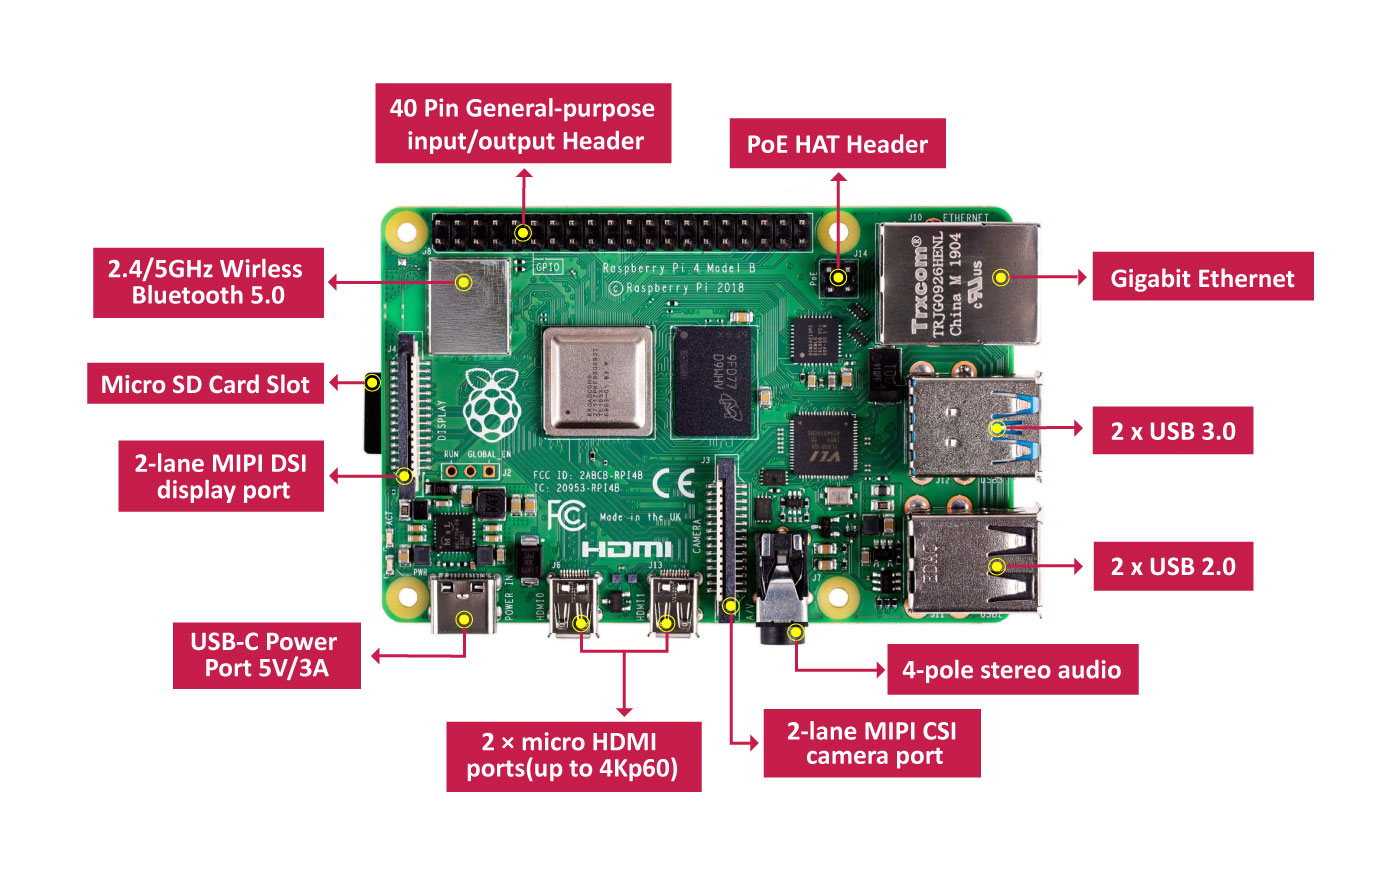
\includegraphics[width = 0.8\textwidth]{Caps/Figs/mat-met/raspberryPI.jpg}
   \label{fig:RaspberryPi-CAM}
    \fonte{Site\protect\footnotemark}
\end{figure}
\footnotetext{Disponível em: \url{https://raw.githubusercontent.com/SeeedDocument/Raspberry-Pi-4/master/img/hardware-overview-1400.jpg}. Acesso em: 8 set. 2020.}

\nomenclature{HDMI}{High-Definition Multimedia Interface}

%================================================================================
\section{Robô Móvel}
\label{sec:robomovel}

Os robôs estão presentes no dia a dia da humanidade de diversas formas, seja ela em processos industriais, residências ou internet bot (softwares para simulação de ação humana). Ao longo dos últimos anos o interesse está em volta dos RMAs, capazes de identificar e se deslocar no ambiente que estão inseridos. Estes são classificados de acordo com o meio em que se movem, sendo ele terrestre, subaquático ou aéreo.

Quando se projeta um robô móvel deve se considerar o tipo de ambiente que ele atuará \cite{rogeralex1999}. Estes ambientes são classificados em estruturados, semi-estruturados e não-estruturados. Em um ambiente estruturado, o robô tem conhecimento prévio da quantidade e localização dos objetos. Logo, um ambiente que não é alterado, resultando em um mapa fixo de rotas possíveis do robô. Um ambiente semi-estruturado é considerado fechado e possui terreno não acidentado, mas seus limites são desconhecidos. Por fim, em um ambiente não-estruturado, o robô não possui nenhum conhecimento a respeito dos objetos ou terreno, podendo ser constantemente modificado. Exige-se então um robô com maior autonomia, capaz de se adequar ao ambiente dinâmico.

Os RMAs tem como características fundamentais as capacidades de locomoção e de operação de modo semi ou completamente autônomo. Também deve ser considerado que maiores níveis de autonomia serão alcançados somente à medida que o robô passe a integrar outros aspectos considerados de maior importância, como: capacidade de percepção (sensores que conseguem "ler" o ambiente onde ele atua), capacidade de agir (atuadores e motores capazes de produzir ações, tais como o deslocamento do robô no ambiente), robustez e inteligência (capacidade de lidar com as mais diversas situações, de modo a resolver tarefas por mais complexas que sejam) \cite{wolf2009robotica}.

%================================================================================
\section{Sensores}
\label{sec:sensores}

Um sensor pode ser definido como um dispositivo projetado para quantificar ou detectar parâmetros específicos por meio de elementos transdutores \cite{rogeralex1999}. 
Múltiplos sensores são utilizados em RMAs para o aumento de seu nível de autonomia, neste trabalho serão utilizados sensores ultrassônicos e um sensor de imagem para visão artificial.

Os sensores individualmente fornecem apenas uma "visão de mundo", parcial, incompleta e sujeita a erros, sendo papel do sistema de controle adquirir, unificar e tratar estas informações de forma robusta e inteligente \cite{wolf2009robotica}.

\subsection{Sensores Ultrassônicos}
\label{subsec:sensores-ultrassônicos}

Os sensores ultrassônicos emitem energia sonora em cones, conforme a Figura~\ref{fig:sensor-ultrassonico}, e sua diretividade depende do ângulo de abertura deste cone. É formado por um emissor e um receptor dispostos tanto juntos como separados, dependendo da configuração desejada. É o princípio de um sonar.

\begin{figure}[!hbtp]
  \centering
   \caption{Sensor Ultrassônico}
    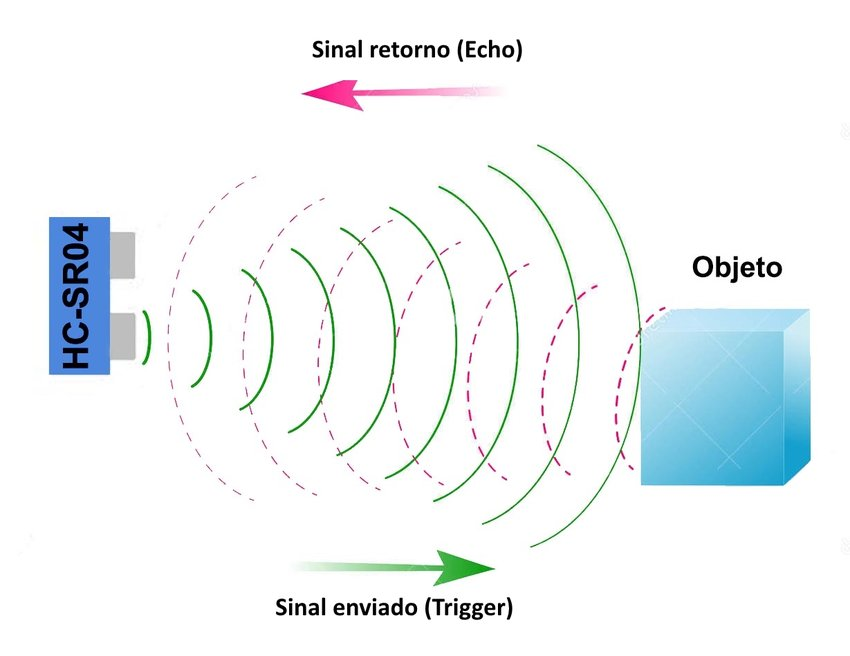
\includegraphics[width = 0.8\textwidth]{Caps/Figs/mat-met/ultrassonico.jpg}
   \label{fig:sensor-ultrassonico}
    \fonte{Site\protect\footnotemark}
\end{figure}
\footnotetext{Disponível em: \url{https://www.researchgate.net/figure/Figura-4-Funcionamento-do-sensor-ultrassonico-HC-SR04-Fonte-Site-Filipeflop-2_fig4_331135149}. Acesso em: 8 set. 2020.}

\subsection{Sensor de Imagem Utilizando Visão Artificial}
\label{subsec:sensores-imagensVisão}

A visão é o sentido mais poderoso e complexo do ser humano. É através dela que ele recebe uma grande quantidade de informações a respeito do mundo que o cerca, o que facilita interagir inteligentemente com o ambiente dinâmico. Utilizando informações visuais, o homem é capaz de estimar a posição de objetos (relativa a ele mesmo ou relativa a outros objetos), identificar formas, perceber movimentos e estimar dimensões. Tudo isso sem contato direto com os objetos \cite{rogeralex1999}.
Constantemente, há o empenho de pesquisadores para prover aos RMAs um sistema de sensoriamento capaz de desempenhar as funções da visão humana, porém ainda estão longe de obter a precisão e velocidade de processamento de informações.

Um sensor de imagem, comporta-se como a retina dos olhos, capta a luminosidade das imagens que são projetadas sobre ele continuamente e dá início ao processo de captura de uma instância ou de uma sequência de instâncias da imagem consecutivamente. Trata-se de um chip que pode contar com dezenas de milhões de transdutores fotossensíveis, cada um deles é capaz de converter a energia luminosa de um ponto da imagem em carga elétrica para ser lida ou gravada posteriormente na forma de imagem digitalizada em valores numéricos. Na Figura~\ref{fig:sensor-camRaspberry} tem-se um exemplo de câmera compatível com Raspberry Pi. 

\begin{figure}[!hbtp]
  \centering
   \caption{Câmera compatível com Raspberry Pi}
    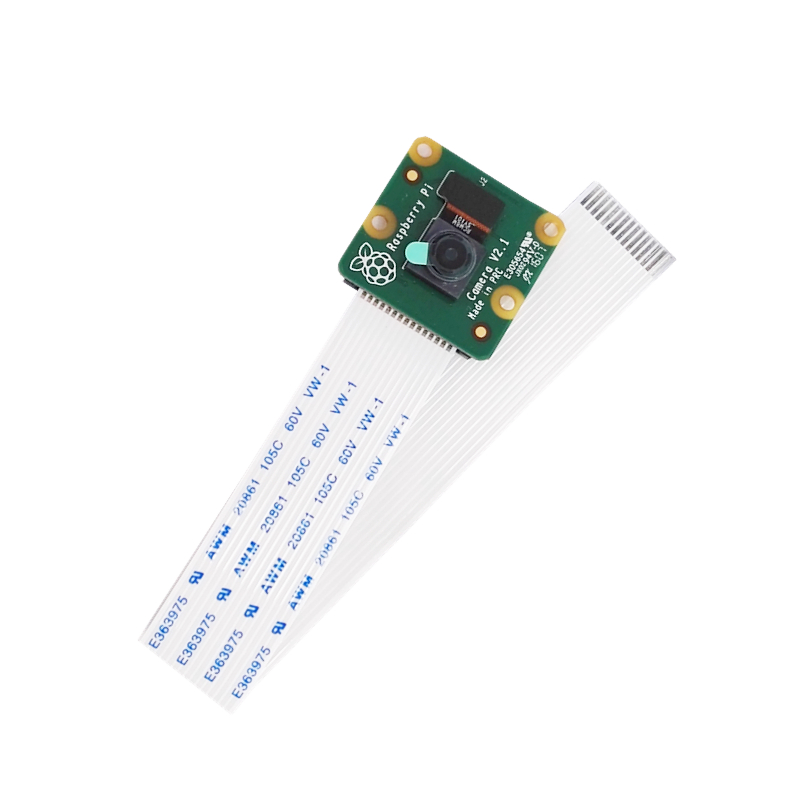
\includegraphics[width = 0.8\textwidth]{Caps/Figs/mat-met/CamRaspberry.jpg}
   \label{fig:sensor-camRaspberry}
    \fonte{Site\protect\footnotemark}
\end{figure}
\footnotetext{Disponível em: \url{https://uploads.filipeflop.com/2017/07/New-Raspberry-Pi-Camera-V2-Video-Module-8MP.jpg}. Acesso em: 8 set. 2020.}

Visão computacional é definida como sendo o conjunto de técnicas computacionais que estimam ou explicitam as propriedades geométricas e dinâmicas do mundo tridimensional a partir de imagens. Trata-se da obtenção automática de informação a respeito do ambiente disponibilizando-a ao sistema de controle, que decidirá qual o comportamento adotar. Utiliza-se de câmeras e plataformas onde essas imagens possam ser processadas, sendo considerado o tipo de informação relevante, a metodologia para extrair a informação e quais as representações empregadas para a atuação do robô.

%================================================================================








 %materiais e métodos
    %\include{Caps/objetivos.tex}
    \chapter{Resultados Esperados}
\label{chap:ResultadosEsperados}

Neste trabalho de conclusão de curso espera-se construir e testar um robô autônomo que seja capaz de navegar buscando marcadores espalhados por um percurso pré-definido. 

O sistema de navegação do robô funcionará através de um algoritmo YOLO para detecção de objetos que informará ao controle do robô onde fica o próximo marco do trajeto. Baseado na informação contida no marcador encontrado, o robô procura o próximo marco e assim sucessivamente até o final da rota.

Para o teste, propõe-se utilizar uma pista inspirada por \citeauthor{memon2015autonomous} (\citeyear{memon2015autonomous}), a qual pode ser vista na Figura~\ref{fig:pista-testes}.

\begin{figure}[!hbtp]
  \centering
   \caption{Pista de testes.}
    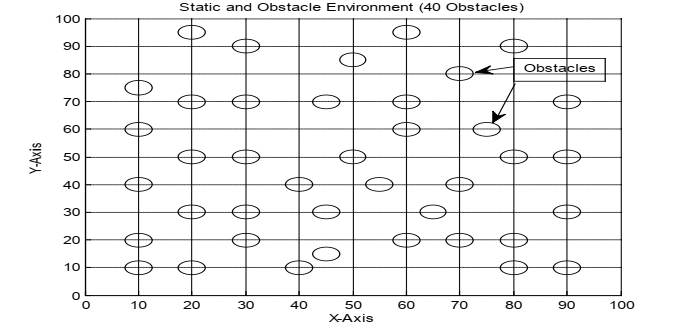
\includegraphics[width = 0.8\textwidth]{Caps/Figs/resultados/pista.png}
   \label{fig:pista-testes}
    \fonte{\cite{memon2015autonomous}}
\end{figure}

Espera-se que o robô consiga desviar de obstáculos de maneira seletiva e mesmo que o ambiente sofra alterações dinâmicas, ainda será possível encontrar uma rota viável. Alterando-se a posição dos objetos dinamicamente o robô conseguirá diferenciar obstáculos de não obstáculos.

O algoritmo de visão computacional será implementado e avaliado sua acurácia para detectar obstáculos em tempo real, durante a movimentação do RMA. O algoritmo de controle desempenhará o papel de planejar as novas trajetórias para a movimentação.

O RMA será prototipado utilizando um Raspberry Pi e um Arduino, onde serão integrados os sensores e atuadores. Este contará com um chassi visto na Figura~\ref{fig:chassi}, motores, rodas, sensores de imagem e ultrassônicos. A programação será realizada em C para o Arduino, pela Arduino IDE, onde será definido sua lógica de movimentação; e em Python para o Raspberry Pi que irá tratar a detecção dos objetos.

Os sensores ultrassônicos atuarão como última ação do RMA, caso o sistema de visão computacional ou o controle de sua trajetória falhe.

\begin{figure}[!hbtp]
  \centering
   \caption{Chassi.}
    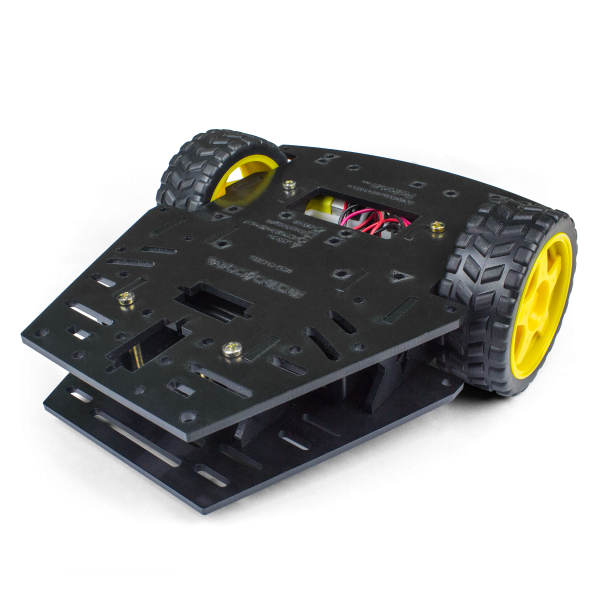
\includegraphics[width = 0.8\textwidth]{Caps/Figs/resultados/582_1_H.png}
   \label{fig:chassi}
    \fonte{Robocore}
\end{figure} %resultados esperados
    % CRONOGRAMA-------------------------------------------------------------------

\chapter{Cronograma}
\label{chap:cronograma}

% Insere uma linha vertical
\noindent\hrulefill

\textbf{Atividades:}
\begin{enumerate}
	\item \textbf{Elaboração da proposta de TCC}: Definição do escopo do projeto e determinação da metodologia.
	\item \textbf{Escrita do texto do TCC 1}: Pesquisa métodos de visão computacional e descrição de todo  processo realizado para a implementação.
	\item \textbf{Agendamento da apresentação do TCC 1}: Agendamento da apresentação do trabalho com o professor orientador.
	\item \textbf{Revisão do texto}: Correção do trabalho escrito e finalização para entrega. 
	\item \textbf{Defesa do TCC 1}: Defesa do trabalho proposto.
	\item \textbf{Alterações e entrega do TCC 1}: Entrega do TCC 1 com as devidas alterações solicitadas pela banca. 	
	\item \textbf{Implementação do algoritmo YOLO}: Será implementado o algoritmo de visão computacional YOLO e embarcado no Raspberry Pi.
	\item \textbf{Implementação do algoritmo de controle}: Será implementado o algoritmo de controle e embarcado no arduino.
	\item \textbf{Montagem do protótipo}: Montagem do chassi do robô e fixação de módulos e placas.
	\item \textbf{Teste do protótipo}: Teste das implementações dos algoritmos e do RMA. Escrita dos resultados.
	\item \textbf{Correção Final}: Correção do trabalho escrito.
	\item \textbf{Defesa do TCC 2}: Defesa do TCC 2. 
\end{enumerate}

Os \autoref{qua:cronograma2020} e \autoref{qua:cronograma2021} mostram o período previsto para as atividades propostas.

\begin{quadro}[!ht]
\centering
\caption{\label{qua:cronograma2020}Cronograma de atividades de 2020}

\begin{tabular}{|c|l|l|l|c|l|}
\hline
\multirow{2}{*}{\textbf{Atividades}} & \multicolumn{5}{c|}{\textbf{2020}}                                                                                                                                    \\ \cline{2-6} 
                                     & \multicolumn{1}{c|}{\textbf{Ago}} & \multicolumn{1}{c|}{\textbf{Set}} & \multicolumn{1}{c|}{\textbf{Out}} & \textbf{Nov}          & \multicolumn{1}{c|}{\textbf{Dez}} \\ \hline
Elaboração da proposta de TCC        & \multicolumn{1}{c|}{x}            &                                   &                                   & \multicolumn{1}{l|}{} &                                   \\ \hline
Escrita do texto do TCC 1            &                                   & \multicolumn{1}{c|}{x}            & \multicolumn{1}{c|}{x}            & x                     &                                   \\ \hline
Agendamento da apresentação do TCC 1 &                                   &                                   & \multicolumn{1}{c|}{x}            & \multicolumn{1}{l|}{} &                                   \\ \hline
Revisão do texto                     &                                   &                                   &                                   & x                     & \multicolumn{1}{c|}{x}            \\ \hline
Defesa do TCC 1                      &                                   &                                   &                                   & x                     &                                   \\ \hline
Alterações e entrega do TCC 1        &                                   &                                   &                                   & x                     & \multicolumn{1}{c|}{x}            \\ \hline
\end{tabular}

\fonte{Autor}
\end{quadro}

%==============================================================================================================================

\begin{quadro}[!ht]
\centering
\caption{\label{qua:cronograma2021}Cronograma de atividades de 2021}

\begin{tabular}{|c|l|c|l|l|l|l|}
\hline
\multirow{2}{*}{\textbf{Atividades}}   & \multicolumn{6}{c|}{\textbf{2021}}                                                                                                                                                                         \\ \cline{2-7} 
                                       & \multicolumn{1}{c|}{\textbf{Jan}} & \textbf{Fev}          & \multicolumn{1}{c|}{\textbf{Mar}} & \multicolumn{1}{c|}{\textbf{Abr}} & \multicolumn{1}{c|}{\textbf{Maio}} & \multicolumn{1}{c|}{\textbf{Jun}} \\ \hline
Implementação do algoritmo YOLO        & \multicolumn{1}{c|}{x}            & x                     &                                   &                                   &                                    &                                   \\ \hline
Implementação do algoritmo de controle &                                   & x                     & \multicolumn{1}{c|}{x}            &                                   &                                    &                                   \\ \hline
Montagem do protótipo                  &                                   & x                     & \multicolumn{1}{c|}{x}            & \multicolumn{1}{c|}{x}            &                                    &                                   \\ \hline
Teste do protótipo                     &                                   & \multicolumn{1}{l|}{} &                                   & \multicolumn{1}{c|}{x}            & \multicolumn{1}{c|}{x}             &                                   \\ \hline
Correção final                         &                                   & \multicolumn{1}{l|}{} &                                   &                                   &                                    & \multicolumn{1}{c|}{x}            \\ \hline
Defesa do TCC 2                        &                                   & \multicolumn{1}{l|}{} &                                   &                                   &                                    & \multicolumn{1}{c|}{x}            \\ \hline
\end{tabular}

\fonte{Autor}
\end{quadro}



% insere o cronograma
%% CRONOGRAMA-------------------------------------------------------------------

\chapter{Cronograma}
\label{chap:cronograma}

% Insere uma linha vertical
\noindent\hrulefill

\textbf{Atividades:}
\begin{enumerate}
	\item \textbf{Elaboração da proposta de TCC}: Definição do escopo do projeto e determinação da metodologia.
	\item \textbf{Escrita do texto do TCC 1}: Pesquisa métodos de visão computacional e descrição de todo  processo realizado para a implementação.
	\item \textbf{Agendamento da apresentação do TCC 1}: Agendamento da apresentação do trabalho com o professor orientador.
	\item \textbf{Revisão do texto}: Correção do trabalho escrito e finalização para entrega. 
	\item \textbf{Defesa do TCC 1}: Defesa do trabalho proposto.
	\item \textbf{Alterações e entrega do TCC 1}: Entrega do TCC 1 com as devidas alterações solicitadas pela banca. 	
	\item \textbf{Implementação do algoritmo YOLO}: Será implementado o algoritmo de visão computacional YOLO e embarcado no Raspberry Pi.
	\item \textbf{Implementação do algoritmo de controle}: Será implementado o algoritmo de controle e embarcado no arduino.
	\item \textbf{Montagem do protótipo}: Montagem do chassi do robô e fixação de módulos e placas.
	\item \textbf{Teste do protótipo}: Teste das implementações dos algoritmos e do RMA. Escrita dos resultados.
	\item \textbf{Correção Final}: Correção do trabalho escrito.
	\item \textbf{Defesa do TCC 2}: Defesa do TCC 2. 
\end{enumerate}

Os \autoref{qua:cronograma2020} e \autoref{qua:cronograma2021} mostram o período previsto para as atividades propostas.

\begin{quadro}[!ht]
\centering
\caption{\label{qua:cronograma2020}Cronograma de atividades de 2020}

\begin{tabular}{|c|l|l|l|c|l|}
\hline
\multirow{2}{*}{\textbf{Atividades}} & \multicolumn{5}{c|}{\textbf{2020}}                                                                                                                                    \\ \cline{2-6} 
                                     & \multicolumn{1}{c|}{\textbf{Ago}} & \multicolumn{1}{c|}{\textbf{Set}} & \multicolumn{1}{c|}{\textbf{Out}} & \textbf{Nov}          & \multicolumn{1}{c|}{\textbf{Dez}} \\ \hline
Elaboração da proposta de TCC        & \multicolumn{1}{c|}{x}            &                                   &                                   & \multicolumn{1}{l|}{} &                                   \\ \hline
Escrita do texto do TCC 1            &                                   & \multicolumn{1}{c|}{x}            & \multicolumn{1}{c|}{x}            & x                     &                                   \\ \hline
Agendamento da apresentação do TCC 1 &                                   &                                   & \multicolumn{1}{c|}{x}            & \multicolumn{1}{l|}{} &                                   \\ \hline
Revisão do texto                     &                                   &                                   &                                   & x                     & \multicolumn{1}{c|}{x}            \\ \hline
Defesa do TCC 1                      &                                   &                                   &                                   & x                     &                                   \\ \hline
Alterações e entrega do TCC 1        &                                   &                                   &                                   & x                     & \multicolumn{1}{c|}{x}            \\ \hline
\end{tabular}

\fonte{Autor}
\end{quadro}

%==============================================================================================================================

\begin{quadro}[!ht]
\centering
\caption{\label{qua:cronograma2021}Cronograma de atividades de 2021}

\begin{tabular}{|c|l|c|l|l|l|l|}
\hline
\multirow{2}{*}{\textbf{Atividades}}   & \multicolumn{6}{c|}{\textbf{2021}}                                                                                                                                                                         \\ \cline{2-7} 
                                       & \multicolumn{1}{c|}{\textbf{Jan}} & \textbf{Fev}          & \multicolumn{1}{c|}{\textbf{Mar}} & \multicolumn{1}{c|}{\textbf{Abr}} & \multicolumn{1}{c|}{\textbf{Maio}} & \multicolumn{1}{c|}{\textbf{Jun}} \\ \hline
Implementação do algoritmo YOLO        & \multicolumn{1}{c|}{x}            & x                     &                                   &                                   &                                    &                                   \\ \hline
Implementação do algoritmo de controle &                                   & x                     & \multicolumn{1}{c|}{x}            &                                   &                                    &                                   \\ \hline
Montagem do protótipo                  &                                   & x                     & \multicolumn{1}{c|}{x}            & \multicolumn{1}{c|}{x}            &                                    &                                   \\ \hline
Teste do protótipo                     &                                   & \multicolumn{1}{l|}{} &                                   & \multicolumn{1}{c|}{x}            & \multicolumn{1}{c|}{x}             &                                   \\ \hline
Correção final                         &                                   & \multicolumn{1}{l|}{} &                                   &                                   &                                    & \multicolumn{1}{c|}{x}            \\ \hline
Defesa do TCC 2                        &                                   & \multicolumn{1}{l|}{} &                                   &                                   &                                    & \multicolumn{1}{c|}{x}            \\ \hline
\end{tabular}

\fonte{Autor}
\end{quadro}



% insere o cronograma
%% CRONOGRAMA-------------------------------------------------------------------

\chapter{Cronograma}
\label{chap:cronograma}

% Insere uma linha vertical
\noindent\hrulefill

\textbf{Atividades:}
\begin{enumerate}
	\item \textbf{Elaboração da proposta de TCC}: Definição do escopo do projeto e determinação da metodologia.
	\item \textbf{Escrita do texto do TCC 1}: Pesquisa métodos de visão computacional e descrição de todo  processo realizado para a implementação.
	\item \textbf{Agendamento da apresentação do TCC 1}: Agendamento da apresentação do trabalho com o professor orientador.
	\item \textbf{Revisão do texto}: Correção do trabalho escrito e finalização para entrega. 
	\item \textbf{Defesa do TCC 1}: Defesa do trabalho proposto.
	\item \textbf{Alterações e entrega do TCC 1}: Entrega do TCC 1 com as devidas alterações solicitadas pela banca. 	
	\item \textbf{Implementação do algoritmo YOLO}: Será implementado o algoritmo de visão computacional YOLO e embarcado no Raspberry Pi.
	\item \textbf{Implementação do algoritmo de controle}: Será implementado o algoritmo de controle e embarcado no arduino.
	\item \textbf{Montagem do protótipo}: Montagem do chassi do robô e fixação de módulos e placas.
	\item \textbf{Teste do protótipo}: Teste das implementações dos algoritmos e do RMA. Escrita dos resultados.
	\item \textbf{Correção Final}: Correção do trabalho escrito.
	\item \textbf{Defesa do TCC 2}: Defesa do TCC 2. 
\end{enumerate}

Os \autoref{qua:cronograma2020} e \autoref{qua:cronograma2021} mostram o período previsto para as atividades propostas.

\begin{quadro}[!ht]
\centering
\caption{\label{qua:cronograma2020}Cronograma de atividades de 2020}

\begin{tabular}{|c|l|l|l|c|l|}
\hline
\multirow{2}{*}{\textbf{Atividades}} & \multicolumn{5}{c|}{\textbf{2020}}                                                                                                                                    \\ \cline{2-6} 
                                     & \multicolumn{1}{c|}{\textbf{Ago}} & \multicolumn{1}{c|}{\textbf{Set}} & \multicolumn{1}{c|}{\textbf{Out}} & \textbf{Nov}          & \multicolumn{1}{c|}{\textbf{Dez}} \\ \hline
Elaboração da proposta de TCC        & \multicolumn{1}{c|}{x}            &                                   &                                   & \multicolumn{1}{l|}{} &                                   \\ \hline
Escrita do texto do TCC 1            &                                   & \multicolumn{1}{c|}{x}            & \multicolumn{1}{c|}{x}            & x                     &                                   \\ \hline
Agendamento da apresentação do TCC 1 &                                   &                                   & \multicolumn{1}{c|}{x}            & \multicolumn{1}{l|}{} &                                   \\ \hline
Revisão do texto                     &                                   &                                   &                                   & x                     & \multicolumn{1}{c|}{x}            \\ \hline
Defesa do TCC 1                      &                                   &                                   &                                   & x                     &                                   \\ \hline
Alterações e entrega do TCC 1        &                                   &                                   &                                   & x                     & \multicolumn{1}{c|}{x}            \\ \hline
\end{tabular}

\fonte{Autor}
\end{quadro}

%==============================================================================================================================

\begin{quadro}[!ht]
\centering
\caption{\label{qua:cronograma2021}Cronograma de atividades de 2021}

\begin{tabular}{|c|l|c|l|l|l|l|}
\hline
\multirow{2}{*}{\textbf{Atividades}}   & \multicolumn{6}{c|}{\textbf{2021}}                                                                                                                                                                         \\ \cline{2-7} 
                                       & \multicolumn{1}{c|}{\textbf{Jan}} & \textbf{Fev}          & \multicolumn{1}{c|}{\textbf{Mar}} & \multicolumn{1}{c|}{\textbf{Abr}} & \multicolumn{1}{c|}{\textbf{Maio}} & \multicolumn{1}{c|}{\textbf{Jun}} \\ \hline
Implementação do algoritmo YOLO        & \multicolumn{1}{c|}{x}            & x                     &                                   &                                   &                                    &                                   \\ \hline
Implementação do algoritmo de controle &                                   & x                     & \multicolumn{1}{c|}{x}            &                                   &                                    &                                   \\ \hline
Montagem do protótipo                  &                                   & x                     & \multicolumn{1}{c|}{x}            & \multicolumn{1}{c|}{x}            &                                    &                                   \\ \hline
Teste do protótipo                     &                                   & \multicolumn{1}{l|}{} &                                   & \multicolumn{1}{c|}{x}            & \multicolumn{1}{c|}{x}             &                                   \\ \hline
Correção final                         &                                   & \multicolumn{1}{l|}{} &                                   &                                   &                                    & \multicolumn{1}{c|}{x}            \\ \hline
Defesa do TCC 2                        &                                   & \multicolumn{1}{l|}{} &                                   &                                   &                                    & \multicolumn{1}{c|}{x}            \\ \hline
\end{tabular}

\fonte{Autor}
\end{quadro}



% insere o cronograma
%\input{dados/quadros/cronograma/crono.tex}


 %cronograma
    \bibliography{references}
    
\end{document}
